\documentclass{article}[a4paper,12pt]
\usepackage{pst-knot} % For drawing knots
\usepackage{graphicx} % For including images
\usepackage{amsmath} % For math typesetting if needed
\usepackage{amssymb} % For mathfrak if used for H
\usepackage{hyperref} % For clickable URLs and cross-references
\hypersetup{
    colorlinks=true,
    linkcolor=blue,
    filecolor=magenta,
    urlcolor=cyan,
    pdftitle={Knots, Arithmetic Torsion, and Cyclotomic Fields},
    pdfpagemode=FullScreen,
    }

\title{Knots, Arithmetic Torsion, and Cyclotomic Fields}
\author{Mingli Yuan, Gemini, ChatGPT}
\date{\today}

\begin{document}

\maketitle

\begin{abstract}
This document explores an arithmetic interpretation of knot group theory, focusing on the relationship between knot relators, their corresponding Alexander polynomials, and a newly defined measure termed global arithmetic torsion. By mapping knot group generators to specific arithmetic operations involving a parameter $t$, we demonstrate how the closure condition of a relator path can yield the Alexander polynomial equation $\Delta(t)=0$. Furthermore, the global arithmetic torsion of such paths, $\tau(\gamma_R)(t)$, exhibits a remarkable structure, consistently factoring into the Alexander polynomial $\Delta(t)$ and a cyclotomic component of the form $t^K-1$. This suggests a deep connection between knot topology, the non-commutative nature of arithmetic operation sequences, and algebraic properties related to roots of unity and cyclotomic fields. Examples, including the figure-eight knot ($4_1$) and knots $6_2$ and $6_3$, are used to illustrate these findings.
\end{abstract}

\section{Introduction}

Knot theory, a branch of topology, studies mathematical knots, which are embeddings of a circle in 3-dimensional Euclidean space. A fundamental invariant associated with a knot is its Alexander polynomial, $\Delta(t)$, a Laurent polynomial in a variable $t$ with integer coefficients. Knot groups, the fundamental groups of knot complements, provide another powerful algebraic invariant. These groups are often presented in terms of generators and relators.

This work investigates an arithmetic interpretation of knot group operations. By mapping the generators of a knot group to specific arithmetic operations (typically multiplication by a parameter $t$ and addition of unity) acting within an arithmetic expression space, we can translate knot group relators into sequences of arithmetic operations, forming what we call "relator paths." The condition that such a path corresponds to the identity element in the knot group imposes constraints on the parameter $t$.

A key concept explored herein is ``arithmetic torsion.'' Arithmetic operations, such as addition and multiplication, are fundamental. When sequenced, their order of application can significantly alter the outcome; for instance, $(x+c_1) \cdot t \neq (x \cdot t) + c_1$ in general. This failure to commute is a basic form of non-commutativity. For a simple pair of operations, this effect can be quantified locally. When considering an entire path composed of a sequence of arithmetic operations, these non-commutative effects can accumulate.

We introduce \textbf{global arithmetic torsion}, denoted $\tau(\gamma)$, for a given arithmetic path $\gamma$. It is defined as the difference between the standard evaluation of the path, $\nu(\gamma)$, and the evaluation of a "reversed-sequence path," $\nu(\bar{\gamma})$, where the literal operations of $\gamma$ are applied in the exact reverse order:
\[ \tau(\gamma)(t) = \nu(\gamma)(t) - \nu(\bar{\gamma})(t) \]
A vanishing global arithmetic torsion, $\tau(\gamma)(t)=0$, implies that the path $\gamma$ and its reversed-sequence counterpart $\bar{\gamma}$ yield the same result under evaluation with parameter $t$, suggesting an "effective commutativity" for the overall path under these specific conditions.

This document demonstrates through examples that for paths $\gamma_R$ derived from knot relators:
\begin{enumerate}
    \item The condition for the path to effectively act as identity often leads directly to the Alexander polynomial equation $\Delta(t)=0$.
    \item The global arithmetic torsion $\tau(\gamma_R)(t)$ for these paths exhibits a consistent structure, often factoring into $\Delta(t)$ and a term $t^K-1$, where $K$ is an integer. This latter term brings roots of unity and cyclotomic fields into the picture, providing additional conditions under which the torsion vanishes.
\end{enumerate}
These findings suggest a novel link between knot topology, the algebraic structure of arithmetic operations, and number-theoretic concepts.

\section{Arithmetic Interpretation of Knot Relators and the Alexander Polynomial: The $4_1$ Knot Example}

The figure-eight knot, denoted $4_1$, is a fundamental example in knot theory. Its group presentation can be given with:
\begin{itemize}
    \item Generators: $a, b$
    \item Relator: $abbbaBAAB = 1$ (where $A=a^{-1}, B=b^{-1}$)
    \item Alexander polynomial: $\Delta_{4_1}(t) = t^2 - 3t + 1$
\end{itemize}

\begin{figure}[h]
    \centering
    \begin{pspicture}(-2,-2)(2,2)
        \psKnot[linewidth=3pt,linecolor=blue](0,0){4-1} % Draws the 4_1 knot
    \end{pspicture}
    \caption{The Figure-Eight Knot ($4_1$)}
    \label{fig:knot_4_1}
\end{figure}

In the framework of arithmetic expression geometry, we can interpret the generators and their inverses as operators acting within an arithmetic expression space $\mathfrak{H}$. We establish the following mapping, linking the knot group structure to arithmetic operations involving an indeterminate variable $t$ (associated with the Alexander polynomial):
\begin{itemize}
    \item $a \mapsto \otimes_t$ (multiplication by $t$)
    \item $b \mapsto \oplus_1$ (addition of 1)
    \item $A = a^{-1} \mapsto \oslash_t$ (division by $t$, i.e., multiplication by $t^{-1}$)
    \item $B = b^{-1} \mapsto \ominus_1$ (subtraction of 1)
\end{itemize}
Under this interpretation, the relator $abbbaBAAB$ corresponds to a closed loop path (a specific threadlike expression) in the space $\mathfrak{H}$.

\begin{figure}[h]
    \centering
    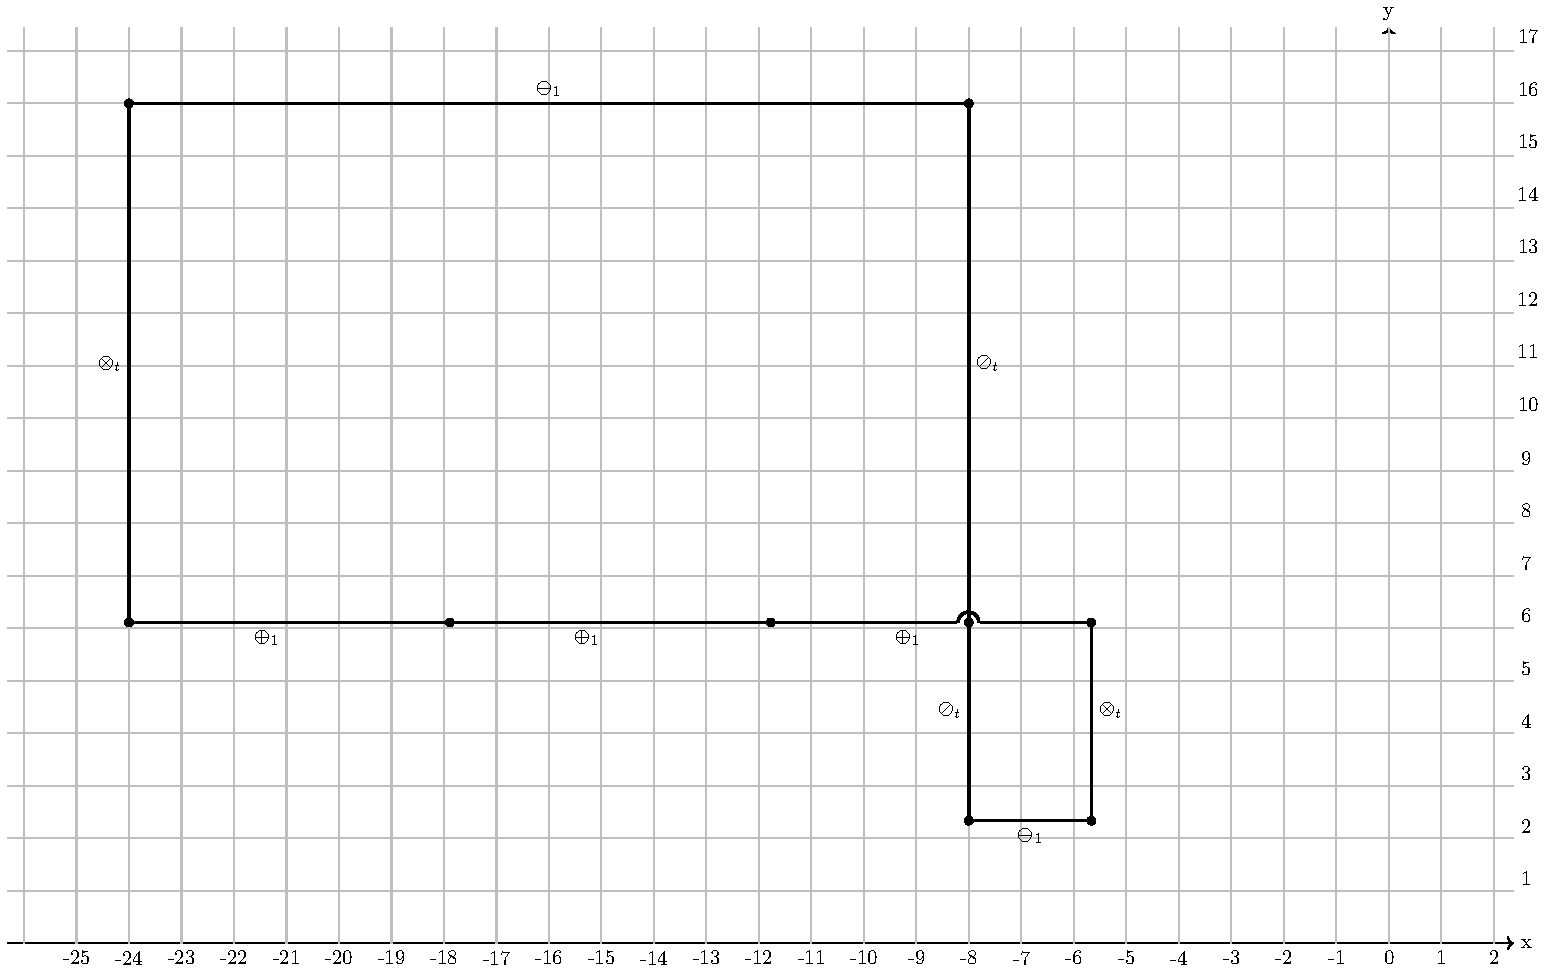
\includegraphics[width=0.8\textwidth]{images/knot_4_1}
    \caption{Schematic representation of the relator path in the arithmetic expression space $\mathfrak{H}$}
    \label{fig:relator}
\end{figure}

Applying the sequence of operators corresponding to the relator $abbbaBAAB$ to a real number $x$ (acting from right to left, consistent with function composition) yields:
\begin{align*}
    \text{Result} &= a(b(b(b(a(B(A(A(B(x))))))))) \\
    &= (x - 1) - t^2 + 3t \\
    &= x - (t^2 - 3t + 1)
\end{align*}
Since the relator $abbbaBAAB$ is equal to the identity element in the knot group, the corresponding path acting on $x$ must return $x$. Therefore, we must have:
\[
x - (t^2 - 3t + 1) = x
\]
This forces the condition $t^2 - 3t + 1 = 0$, which is precisely the Alexander polynomial $\Delta_{4_1}(t)$ of the knot $4_1$ set to zero.

\subsection{Computational Verification for Other Knots}

This observed connection between the knot relator (interpreted arithmetically) and the Alexander polynomial equation $\Delta(t)=0$ is not unique to the knot $4_1$. As previously noted, computational checks for knots up to 11 crossings have verified this direct correspondence for a significant number of knots, including $4_1, 6_2, 6_3, 7_6, 7_7, 8_2, 8_9, 8_{10}, 8_{12}, 9_{11}, 9_{17}, 9_{26}, 9_{27}, 9_{42}, 9_{44}$, and many others. This suggests a potentially deeper underlying pattern.


\section{Global Arithmetic Torsion of Knot Relator Paths}
\label{sec:global_torsion}

Building on the arithmetic interpretation, we can analyze the structure of relator paths further using the concept of global arithmetic torsion.

\subsection{Definition and Observed General Structure}

Let $\gamma_R$ be the arithmetic path corresponding to a knot relator $R$. We define its standard evaluation (starting from an initial value of 0, with multiplicative parameter $t$) as $p(t) = \nu(\gamma_R)(0,t)$. Let $\bar{\gamma}_R$ be the path where the literal sequence of operations from $\gamma_R$ is applied in the exact reverse order, with evaluation $q(t) = \nu(\bar{\gamma}_R)(0,t)$.

The \textbf{global arithmetic torsion} for $\gamma_R$ is:
\[ \tau(\gamma_R)(t) = p(t) - q(t) \]
Based on our computed examples, $p(t)$ and $q(t)$ can often be expressed in the form $p(t) = \sigma_p \Delta(t)/t^{k_p}$ and $q(t) = \sigma_q \Delta(t)/t^{k_q}$, where $\Delta(t)$ is the Alexander polynomial, $k_p, k_q$ are non-negative integers, and $\sigma_p, \sigma_q \in \{+1, -1\}$. In the examples we have analyzed, it has been observed that $\sigma_p = \sigma_q = \sigma_{\text{common}}$. Thus, the torsion can be written as:
\begin{equation} \label{eq:torsion_direct_form}
\tau(\gamma_R)(t) = \sigma_{\text{common}} \Delta(t) \left( \frac{1}{t^{k_p}} - \frac{1}{t^{k_q}} \right)
\end{equation}
This expression naturally becomes zero if $k_p=k_q$.

This torsion often reveals a further structure involving the Alexander polynomial $\Delta(t)$ and a cyclotomic factor. Specifically, it can be rewritten (when $k_p \neq k_q$) in the form:
\begin{equation} \label{eq:torsion_factored_form}
\tau(\gamma_R)(t) = \sigma_{\text{eff}} \cdot \frac{\Delta(t)(t^K-1)}{t^{\max(k_p, k_q)}}
\end{equation}
where:
\begin{itemize}
    \item $\Delta(t)$ is the Alexander polynomial of the knot.
    \item $K = |k_q - k_p|$ is the "degree of the cyclotomic part" of the torsion.
    \item The term $t^K-1$ is the "cyclotomic factor." If $K=0$ (i.e., $k_p=k_q$), this term is zero, making $\tau(\gamma_R)(t) \equiv 0$, consistent with eq.~\eqref{eq:torsion_direct_form}.
    \item $\sigma_{\text{eff}} \in \{+1, -1\}$ is an effective sign factor. Specifically, $\sigma_{\text{eff}} = \sigma_{\text{common}}$ if $k_q > k_p$, and $\sigma_{\text{eff}} = -\sigma_{\text{common}}$ if $k_p > k_q$ (for $K \neq 0$).
\end{itemize}
This structure implies that $\tau(\gamma_R)(t)$ vanishes if:
\begin{enumerate}
    \item $\Delta(t)=0$ (the knot-theoretic condition), OR
    \item $t^K-1=0$ (for $K>0$), meaning $t$ is a $K^{th}$ root of unity (the cyclotomic condition).
\end{enumerate}

\subsection{Illustrative Examples}

Let's examine this structure with the knots $6_2$ and $6_3$.

\subsubsection{Knot $6_2$}
For knot $6_2$, the Alexander polynomial is $\Delta_{6_2}(t) = t^4 - 3t^3 + 3t^2 - 3t + 1$.
Using the standard mapping (generator for '$t$' multiplicative, other generator additive $\oplus_1$), our calculations show:
\begin{itemize}
    \item $p(t) = \nu(\gamma_R)(0,t) = -(t^4 - 3t^3 + 3t^2 - 3t + 1) = -\Delta_{6_2}(t)$.
    (Thus, $\sigma_{\text{common}}=-1, k_p=0$)
    \item $q(t) = \nu(\bar{\gamma}_R)(0,t) = \frac{-(t^4 - 3t^3 + 3t^2 - 3t + 1)}{t^4} = -\frac{\Delta_{6_2}(t)}{t^4}$.
    (Thus, $k_q=4$)
\end{itemize}
Here, $K = |4-0| = 4$, $\max(k_p,k_q)=4$. Since $k_q > k_p$, $\sigma_{\text{eff}} = \sigma_{\text{common}} = -1$.
The Global Arithmetic Torsion, by eq.~\eqref{eq:torsion_direct_form}, is $\tau(\gamma_R)(t) = -\Delta_{6_2}(t)(1 - 1/t^4) = -\frac{\Delta_{6_2}(t)(t^4-1)}{t^4}$.
This matches the factored form with $\sigma_{\text{eff}}=-1$. The torsion vanishes if $\Delta_{6_2}(t)=0$ or if $t^4-1=0$.

\subsubsection{Knot $6_3$}
For knot $6_3$, the Alexander polynomial is $\Delta_{6_3}(t) = t^4 - 3t^3 + 5t^2 - 3t + 1$.
Using the standard mapping, our calculations show:
\begin{itemize}
    \item $p(t) = \nu(\gamma_R)(0,t) = t^4 - 3t^3 + 5t^2 - 3t + 1 = \Delta_{6_3}(t)$.
    (Thus, $\sigma_{\text{common}}=1, k_p=0$)
    \item $q(t) = \nu(\bar{\gamma}_R)(0,t) = \frac{t^4 - 3t^3 + 5t^2 - 3t + 1}{t^4} = \frac{\Delta_{6_3}(t)}{t^4}$.
    (Thus, $k_q=4$)
\end{itemize}
Here, $K = |4-0| = 4$, $\max(k_p,k_q)=4$. Since $k_q > k_p$, $\sigma_{\text{eff}} = \sigma_{\text{common}} = 1$.
The Global Arithmetic Torsion, by eq.~\eqref{eq:torsion_direct_form}, is $\tau(\gamma_R)(t) = \Delta_{6_3}(t)(1 - 1/t^4) = \frac{\Delta_{6_3}(t)(t^4-1)}{t^4}$.
This matches the factored form with $\sigma_{\text{eff}}=1$. The torsion vanishes if $\Delta_{6_3}(t)=0$ or if $t^4-1=0$.

\section{Discussion and Future Directions}

The empirical evidence presented, including the initial $4_1$ knot example and the subsequent analysis of global arithmetic torsion for knots like $6_2$ and $6_3$ (and others we have computed like $7_6, 7_7, 8_2, 8_9, 8_{10}, 8_{12}, 9_{11}, 9_{17}, 9_{26}, 9_{27}, 9_{42}, 9_{44}$), strongly suggests a multi-layered connection between knot theory and arithmetic expression geometry.

Firstly, the arithmetic interpretation of knot relators directly links the condition for a relator path to act as identity to the vanishing of the Alexander polynomial $\Delta(t)=0$. This provides an operational method to derive the Alexander polynomial constraint.

Secondly, the concept of global arithmetic torsion, $\tau(\gamma_R)(t) = p(t) - q(t)$, reveals a deeper structure. As shown by eq.~\eqref{eq:torsion_direct_form} and often re-expressed as eq.~\eqref{eq:torsion_factored_form}, this torsion systematically involves the Alexander polynomial $\Delta(t)$ and a cyclotomic factor $t^K-1$ (where $K = |k_q-k_p|$). This means the torsion vanishes not only when $\Delta(t)=0$ but also when $t$ is a $K^{th}$ root of unity (for $K>0$). The appearance of this cyclotomic factor $t^K-1$ (whose factors are products of cyclotomic polynomials $\Phi_d(t)$) strongly indicates a profound link with cyclotomic fields.

The vanishing of torsion implies a type of "effective commutativity" for the evaluated path $\gamma_R$ relative to its reverse-sequence counterpart $\bar{\gamma}_R$. The fact that this occurs precisely when $t$ corresponds to roots of $\Delta(t)$ or to roots of unity points towards significant underlying principles. The intuition that these phenomena might be geometrically related to "some kind of rotation" is compelling, especially since roots of unity define discrete rotational symmetries in the complex plane. When the multiplicative parameter $t$ assumes one of these values, the operator $\otimes_t$ itself embodies this specific rotational symmetry. It is plausible that this inherent symmetry in the multiplicative operations, under these specific values of $t$, leads to a cancellation of non-commutative effects across the entire path $\gamma_R$ when compared to $\bar{\gamma}_R$, resulting in zero global torsion.

Future research could aim to:
\begin{itemize}
    \item Develop a formal geometric model for the arithmetic expression space $\mathfrak{H}^{(t)}$ that could provide a geometric interpretation for $p(t)$, $q(t)$, the torsion $\tau(\gamma_R)(t)$, and the significance of the parameter $t$.
    \item Understand from first principles (e.g., from the relator's symbolic structure and the chosen mapping) how the integers $k_p$, $k_q$, and the sign factors $\sigma_p, \sigma_q$ (and thus $\sigma_{\text{eff}}$) are determined for any given knot.
    \item Explore the conditions under which the Alexander polynomial $\Delta(t)$ appears as a factor in the torsion, and why the specific cyclotomic factor $t^K-1$ emerges. This includes further investigation of cases where $K=0$ (e.g., knots $8_9, 8_{10}$ in our broader survey), leading to identically zero torsion, and what this implies about the symmetry of those specific relator paths under their respective mappings.
\end{itemize}
This arithmetic framework appears to offer a novel lens through which to explore the rich interplay between knot topology, group theory, and algebraic number theory.

\section{Computational Verification Code}

The SageMath script used for the computational verification and calculation of $p(t)$, $q(t)$, and the torsion factors for the knots discussed can be found at:
\url{https://github.com/mountain/knot-alexander/blob/main/torsion.py}

\end{document}